% template for a task
% each task should be added to exactly one workpackage
% in the workpackage task list
\begin{task}[
  title=Reproducible photon science workflows at European XFEL,
  id=reproducibility-xfel,
  lead=XFEL,
  PM=36,
  wphases={7-48},
  partners={INSERM,SRL,UPSUD,EGI}
  ]

\textbf{Summary}

  European XFEL is a research facility that provides X-ray Free
  Electron Laser (XFEL) light to image structures at the nanoscale. It
  is currently the world's most brilliant laser, created in a 3.4km
  long tunnel, and supporting user experiments since September
  2017. These imaging capabilities from European XFEL and similar
  services from synchrotron and neutron sources, underpin lots of
  fundamental and applied research, in domains ranging from fundamental
  physics and material science to biochemistry and drug design. Some
  example data is shown in figure \ref{fig:photon-science-example}.

  All of the data recorded at European XFEL will be made freely
  available after an embargo period of three years
  \cite{EuXFEL-datapolicy-2017}. This provides scientific transparency
  and is expected to enable better exploitation of the data, as more
  researchers than those conducting the experiments have access to the
  results. If the analysis steps are not carefully recorded, there is a risk
  that the necessary understanding of the data is lost by the time it
  is made public or subsequently, greatly reducing its scientific
  value.

  We are keen to complement this open data access to the actual data
  with open access to reproducible data analysis, to confirm
  conclusions drawn and to significantly lower the barriers for
  re-analysis with new tools or for new research purposes.

  A task in the EC funded project Photon and Neutron Open Science
  Cloud (PaNOSC) is using the Jupyter Ecosystem tools as they are in
  2019 to provide interactive data analysis services to complement the
  data: through use of Jupyter Notebook and exploitation of the
  mybinder.org service, this activity will reduce the barrier for
  interactively exploring the data, understanding and making use of
  the data, and to do this through a central portal such as EOSC.

  Here, we combine and use the new developments of this
  proposal to enable new qualities of open science services, and to
  demonstrate the potential impact of these improvements for a wide
  set of EOSC services through a demonstrator in Photon Science.

  \medskip

\begin{figure}[tb]
    \centering
    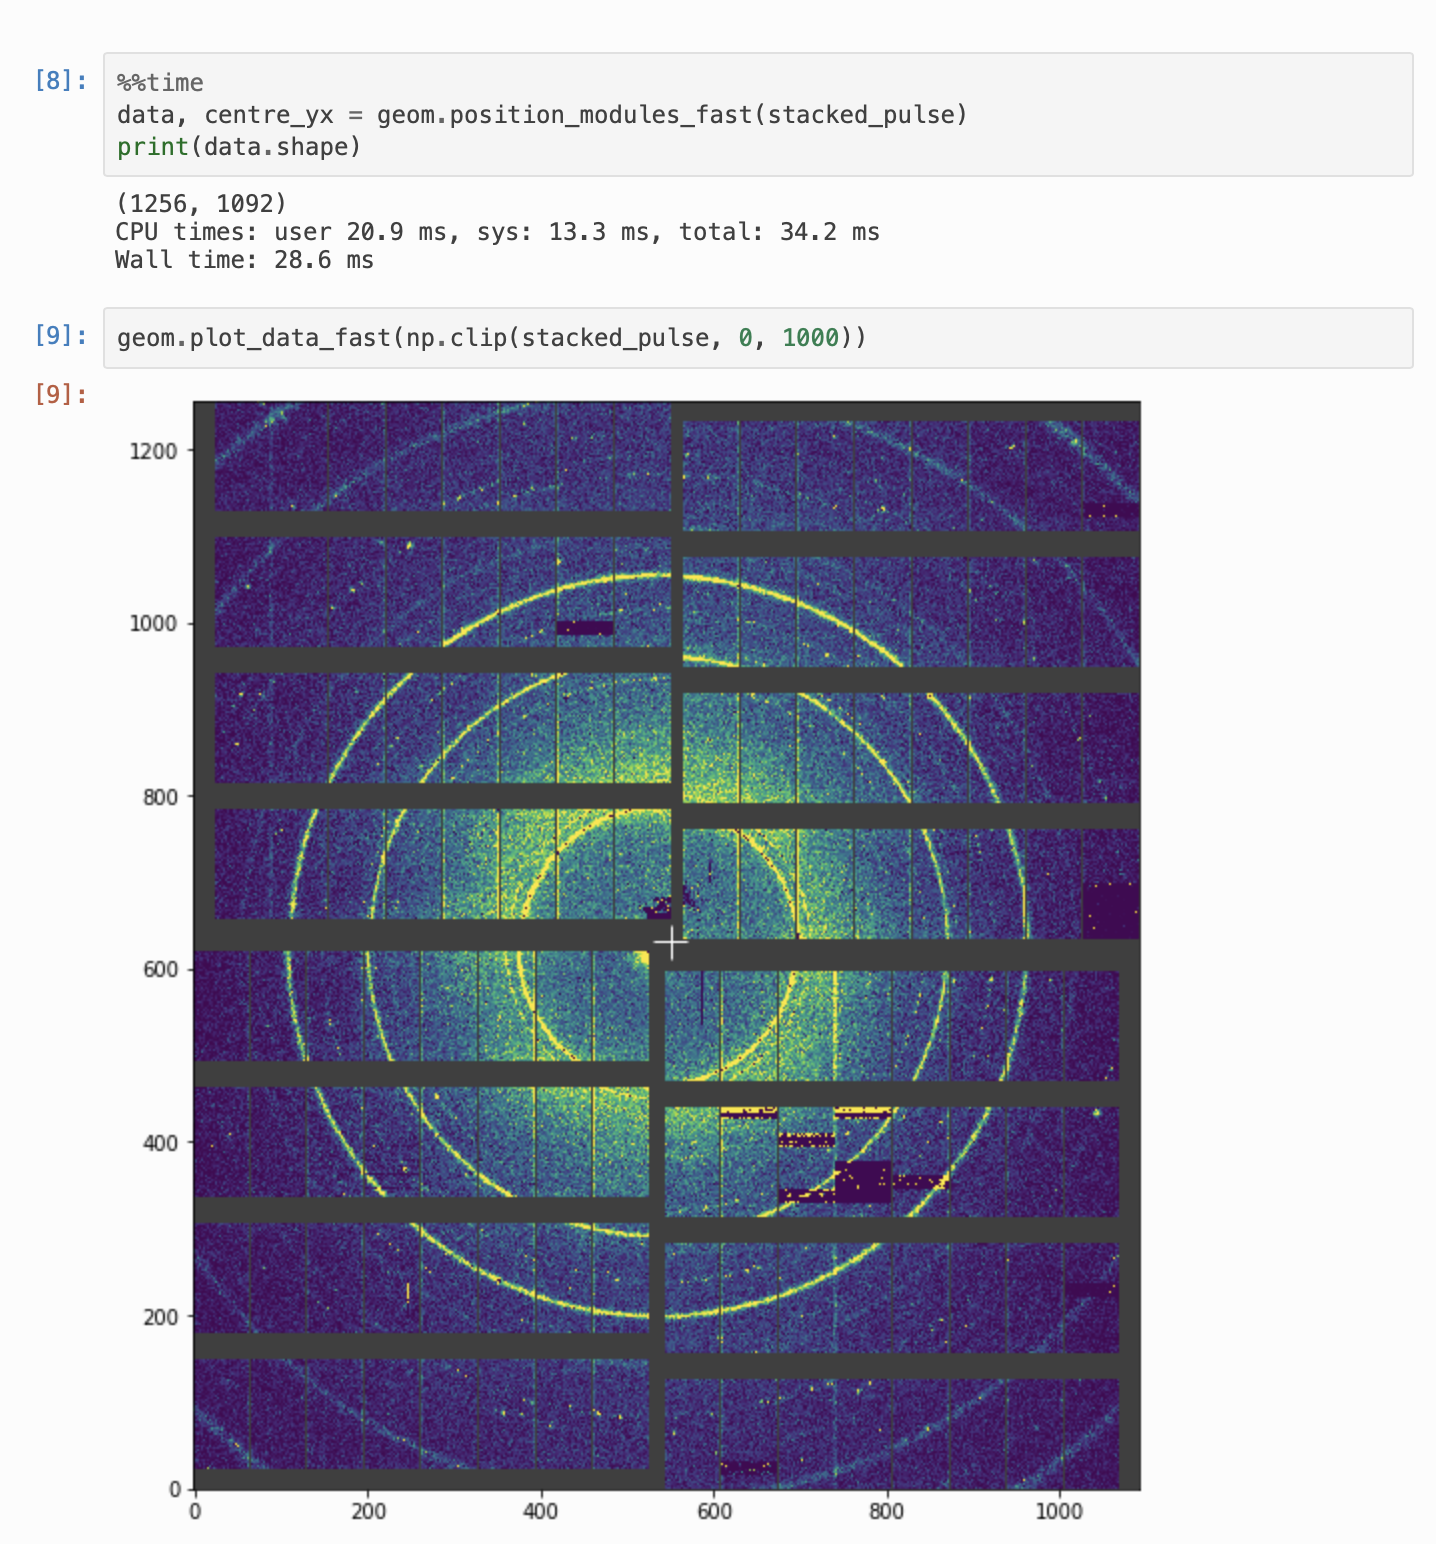
\includegraphics[height=0.3\textheight]{images/photon-science-prototype1.png}
    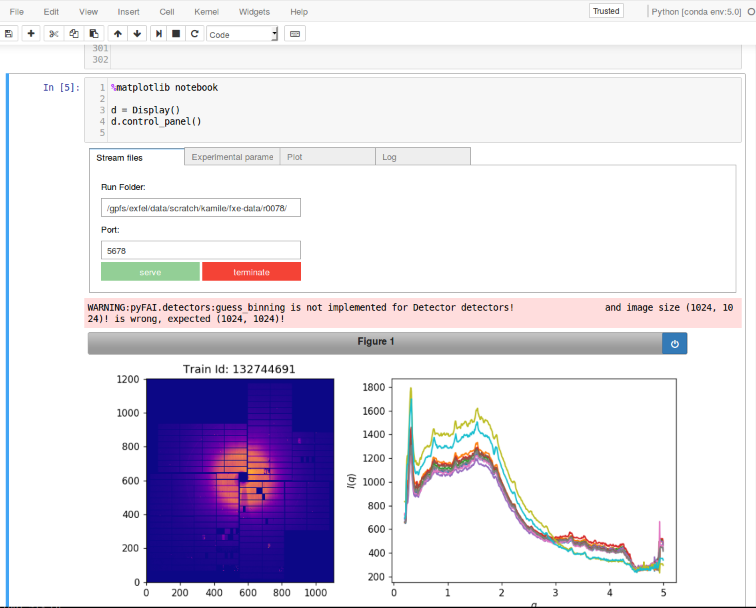
\includegraphics[height=0.3\textheight]{images/photon-science-prototype2.png}
    \caption{Prototypes for data analysis of 2d x-ray detector images
      in the Jupyter notebook, relating to the
      photon science use case.
      % task reference in caption doesn't work
      % \taskref{applications}{reproducibility-xfel}.
      \emph{(Left)} Data from crystallography
      scattering experiment. \emph{(Right)} Azimuthal integration of detector
      data as one step in the data analysis workflow.}
    \label{fig:photon-science-example}
  \end{figure}


  \textbf{Context}

  The very first experiments at European XFEL
  produced as little as 45 terabytes of data on average, but as the
  facility develops, the amount of data produced per time is expected
  to grow substantially: Given the rate of light pulses, there is the
  potential to produce up to a petabyte of data within the beam time
  of one experiment (typically one week). These significant amounts of
  data need to be complemented by complicated workflows to convert the
  data into insight through data analysis. Derived results of such
  data analysis are typically much smaller in size and useful to
  archive together with the raw data. To explain how they have been
  obtained, the particular workflow of data analysis also needs to be
  archived.

  \medskip
  \textbf{Vision}

  At European XFEL we will use Jupyter notebooks to facilitate
  this workflow: the simplest model would be to use one notebook per
  workflow. Once the data capture from the experiment is completed,
  this notebook can be executed (without being displayed in a web
  browser) to start processing the data. When the notebook has
  completed execution, it is saved, and contains the analysis results
  (it may of course also created files on disk as part of the
  process).

  A particularly useful aspect of the notebooks is that they mix data
  analysis commands with outputs, and that the notebook provides a
  complete (and thus reproducible) summary of the data analysis when
  it succeeds with the execution. Should the execution fail, for
  example half-way through the notebook, then derived results obtained
  prior to the error occurring are preserved and can be inspected. The
  error is embedded in the notebook and appears after the command that
  has triggered the error; which helps with debugging the process.

  This is of particular interest as the data analysis processes at
  European XFEL may fail not because of software errors but due to
  variation in the data that require (manual) expert adjustments of
  parameters. The ``failure'' of such an analysis workflow
  (represented through the Notebook) is thus not exceptional, but a
  common occurrence. The scientist conducting the experiment is
  sufficiently skilled to modify the parameters and wants to either
  re-execute the notebook from the beginning or to continue from the
  point of failure. The notebook caters for both use cases. The
  modified notebook would need to be preserved of course to provide
  reproducibility of the derived results that the notebook has
  computed.

  We are aiming for re-executability of the notebook for the lifetime
  of the data. The life time of the archived data at European XFEL is
  currently guaranteed for 5 years and aimed to be 10 years
  \cite{EuXFEL-datapolicy-2017}. It is possible though, that data used
  for publications will be preserved for longer, and it would be
  highly desirable to keep the data analysis re-executable for the
  same period of time, potentially well exceeding 10 years.

  \medskip \textbf{This task}

  This task includes the following activities:
  \begin{compactitem}
  \item Use the software archive for reproducible computation
    (as co-developed in \taskref{ecosystem}{reproducibility}), with
    the aim to provide reproducible computation environments for data analysis at
    European XFEL that remains executable for the same duration as the
    data is kept (currently aiming at 10+ years, at least 5 years).

    As is common in computational science, software used at XFEL often
    relies on specific combinations of libraries, in many cases with
    particular version requirements. Thus we will need a dedicated
    software archive that holds all relevant packages and source codes
    that are required to build the required computational environments
    (see \taskref{ecosystem}{reproducibility}) to ensure they are
    available even if an open source software provider decides to
    remove their repositories, or changes the API of a package, or
    GitHub decides to terminate their business.

    Applying the work from \taskref{ecosystem}{reproducibility} in the
    context of a production system will demonstrate its true utility,
    and provide important feedback for the design. There will be
    iterative feedback and refinement of the service.

  \item Extend the use of notebooks from \emph{interactive} data
    exploration and analysis at European XFEL to also provide
    computational work flows via (semi-)automatic execution of
    notebooks as described above. The work done in
    \taskref{core}{collaboration} will allow us to execute notebooks in
    the background, and to connect to the running notebook process to
    display or inspect progress, or to modify such a notebook if the
    science requires it.

    By doing so, we can make the standard analysis that is carried out
    by the facility available on EOSC as a service. By using one tool
    (the notebook) we simplify processes for users and for the research
    facility.

  \item Use the work from \taskref{ecosystem}{jupyter-widgets} on
    state-preserving widgets to provide GUI-like elements in notebook
    where interactive user input, data exploration or parameter
    modification is required.

  \item Explore use of the Voila capability to provide
    data exploration dash-boards to lower barriers of working with the
    data (will only be possible for somewhat standard experiments).

  \item Work with the PaNOSC project \cite{panosc} to evaluate and use
    these new and EOSC-enabled services for other Photon and Neutron
    Science research facilities.
  \item Develop a demonstrator (Deliverable \localdelivref{xfel-workflows}).

  \item Evaluate the chosen workflow design and experience from using
    it in a real-world context; make this available as a report and
    through presentations/workshops to interested organisations and
    facilities. (\localdelivref{applications-report}).




  \end{compactitem}

 \end{task}
